%\documentclass[Japanese]{dicomopapers}
\documentclass[Japanese,noauthor]{dicomopapers}

\usepackage[dvipdfmx]{graphicx}
\usepackage{latexsym}
\usepackage{bm}
\usepackage{url}

\def\Underline{\setbox0\hbox\bgroup\let\\\endUnderline}
\def\endUnderline{\vphantom{y}\egroup\smash{\underline{\box0}}\\}
\def\|{\verb|}

\def\newblock{\hskip .11em plus .33em minus .07em}

\begin{document}

% 和文表題
\title{圧力センサ搭載ヘルメットを用いた個人識別手法}
% 英文表題
\etitle{DICOMO2020 Paper Format (optional)}

% 所属ラベルの定義
\affiliate{RU}{立命館大学大学院情報理工学研究科}
\affiliate{JST}{国立研究開発法人科学技術振興機構さきがけ}

\author{藤井 敦寛}{ATSUHIRO FUJII}{RU}
\author{村尾 和哉}{KAZUYA MURAO}{RU, JST}

\begin{abstract}
ヘルメットは社会生活において広く利用されている.
%例えば,野球やアメリカンフットボールなどのスポーツ用や二輪車用のヘルメットが存在する.
%工事現場や工場では,作業者は頭部を保護するためにヘルメットを装着することが一般的であり,視線情報を記録可能なウェアラブルカメラを取り付けたヘルメットが販売されている.さらに,通信機能をもつ防災用ヘルメット\cite{disaster_en}が提案されている.このように,さまざまな機能をもつヘルメットがある.
本研究では32個の圧力センサを搭載したヘルメットを装着することで,頭部形状から個人を識別する手法を提案する.提案手法によって,ヘルメット上部に取り付けたディスプレイに名前を表示したり,視線情報などのデータを記録する際に手間なく作業者のラベルを付与できる.また,工場などで役職などにより入室できる部屋が制限されている場合に扉の鍵としても使用できる.
%また,本人認証として用いれば二輪車の鍵としても使用できる.
%鍵として用いる場合,ヘルメットでの本人の識別を挟むため,鍵の盗難による侵入,車両盗難のリスクの減少にも繋がる.
%識別には特徴があり複製が難しいものとして,頭部形状を使用した.
%また,頭部状態の測定にヘルメットを用いている先行研究は筆者らの知る限りは存在しない.
提案手法は,あらかじめデータが登録された複数の人物のうちの1人がヘルメットを装着したときにその人物を識別する個人識別と,ヘルメットを装着した人物が登録者であれば認証し,登録者でなければ拒否する本人認証の2つの機構を備える.
%二輪車の鍵に用いることを想定し,持ち主であるか他人であるかを判別することを目的とする本人認証を行う.
%個人識別では,事前に登録フェーズで教師データとして識別したい利用者全員のデータを蓄積しておき,識別フェーズで得られたセンサ値に対してSupport Vector Machineを用いてベクトルの特徴から識別する.一方,本人認証では事前に登録フェーズで蓄積しておいたバイクの所有者などの認証したい利用者のセンサデータ群と,識別フェーズで得られるセンサ値とのマハラノビス距離を計算し,閾値を用いて認証を行う.
%本手法で用いるデバイス,およびソフトウェアを設計,実装し評価実験を行った.
プロトタイプデバイスと解析用のソフトウェアを実装した後,被験者9人データを採取し,個人識別では精度が100\%,本人認証では被験者全員の平均EERが約7.6\%という結果を得た.
%プロトタイプデバイスは市販のフルフェイス型のヘルメットを加工し圧力センサを取り付け,マイコンに配線することで実装した.解析用のソフトウェアはPythonのscikit-learnを使用して実装した.個人識別ではsklearn.svm.SVCを用いて識別し,sklearn.model\_selection.cross\_val\_scoreを用いて交差検証を行うことで精度を求めるよう設計した.本人認証ではsklearn.covariance.MinCovDetを使用してマハラノビス距離を計算し,閾値を移動しながら評価指標であるFRR,FAR,EERを求めるよう設計した.ソフトウェアを実装した後,評価用に被験者9人からそれぞれ2秒間のセンサ値を20回分収集した.これらのデータセットから個人識別では精度が1.0,本人認証では被験者全員の平均EERが約7.8\%という結果が得られた.
\end{abstract}

% 表題などの出力
\maketitle

% 本文はここから始まる
\section{はじめに}
\label{introduction}
ヘルメットは,スポーツやレジャー,バイク乗車時,工場,災害現場など,社会生活において広く利用されている.これらはいずれも,事故発生時に頭部を保護する目的で着用\cite{helmet}するものであり,頭部との隙間がないことが安全面において重要だとされている.\par

特に,工場や災害現場ではほぼ全員がヘルメットを装着して作業し,短期労働者や業者など,互いに顔を知らないさまざまな人間が出入りしている.一人1個のヘルメットを所有している場合はヘルメットに氏名がテープ等で表示されていため,ヘルメットを装着したままでも遠くからあるいは頭上からでも識別できる.また,作業者によって所持している資格や従事可能な作業が異なるため,所有資格を示すステッカーが販売されており,そのような作業者のヘルメットに貼り付けて識別できるようにしている.しかし,貸与されたヘルメットの場合,ヘルメットに名前が表示されておらず,現場にいる者どうしも誰であるかを判断できず,不審者が容易に侵入できる可能性がある.また,仮に名前が表示されていたとしても,取り間違いによって,作業者とヘルメットの氏名が異なる場合もある.
%行政機関の職員など現場の知識に乏しい人間の出入りの可能性もあり,身分が不明であることは非常に危険であるといえる.
\par

%本研究ではヘルメットの内部に圧力センサを搭載することで,頭部形状から個人を識別する手法を提案する.提案手法によって,ヘルメット上部に取り付けたディスプレイに名前や資格情報を表示できるため,ヘルメットが共用でも互いに認識でき,取り違えることもない.また,ヘルメットに取り付けられたカメラや視線計測装置,各種センサのデータを自動で作業者と紐づけることができる.さらに,GPSや通信機能\cite{disaster_en}\textcolor{red}{通信機能ってなに?}を組み合わせることで,作業員の位置情報を管理できる.さらには,頭部形状を取得することによりヘルメットと頭部の隙間や圧迫の情報を取得できるため,ヘルメットと頭部形状が合っているかを確認することもできる.

本研究ではヘルメットの内部に圧力センサを搭載することで,頭部形状から個人を識別する手法を提案する.提案手法によって,ヘルメット上部に取り付けたディスプレイに名前や資格情報を表示できるため,ヘルメットが共用でも互いに認識でき,取り違えることもない.また,ヘルメットに取り付けられたカメラや視線計測装置,各種センサのデータを自動で作業者と紐づけることができる.さらに,GPSモジュールとアンテナ\cite{disaster_en}を取り付けることで,リアルタイムに作業員の名前と位置情報を送信することができれば,現場の全体の状況が把握しやすくなる.さらには,頭部形状を取得することによりヘルメットと頭部の隙間や圧迫の情報を取得できるため,ヘルメットと頭部形状が合っているかを確認することもできる.

このほか,工場などで役職や資格により入室できる部屋が制限されている場合の扉の鍵としての使用や,バイクの鍵としても使用できる.ヘルメットでの本人識別を行うため,鍵の盗難による侵入,車両盗難のリスクの減少にも繋がる.\par

個人を識別する手法として,パスワードやPIN,ストロークパターンなどの本人がカギを自由に設定できる手法,顔,指紋や筆跡,声紋,光彩などの身体的特徴を用いる手法,筆跡や歩容などの行動的特徴を用いる手法がある.
個人が自由に設定できるパスワードやPIN,ストロークパターンのみを用いて,本研究で想定するような多数の人間の識別を行うことは,パスワードの重複や総当たり攻撃によるなりすましの危険性がある.

身体的特徴に関して,Chenら\cite{face_and_finger}はスマートフォンなどの端末のフロントカメラとリアカメラから得られる顔と指先のビデオ映像からユーザ本人を認証する手法を提案している.ヘルメットの外部にあらかじめカメラを取り付けておくことで装着者を識別できると考えられるが,暗所や雨天では認識精度が低下する恐れがある.また,毎回ヘルメットを被る前に,ヘルメットを持って自身の顔を撮影することは面倒である.
指紋認証\cite{finger_CNN}は,指紋が写真などから容易に複製されるリスクがある.
本研究で用いた頭部形状は,個人ごとに身体的特徴を持つ.また,立体形状であるため複製が困難であると考える.

行動的特徴を使うアプローチの場合,ヘルメットを装着する時点で個人が識別されている必要があるため,ヘルメットを被る動作を特徴とすることも考えられる.筆者らはこれまでにスマートフォンをポケットから取り出す際の加速度センサデータから認証する手法\cite{murao_screen_unlock}を提案した.スマートフォンはポケットや机の上など取る場面が限定されるが,ヘルメットを取る場面は様々であり,この手法をヘルメットに適用することは困難であると考えられる.

以降本稿では,\ref{related}節で関連研究を紹介する.\ref{method}節で提案手法を説明し,\ref{evaluation}節で提案手法の評価実験と結果の考察を行い,最後に\ref{conclude}節で本研究をまとめる.


\section{関連研究}
\label{related}
本節では個人認証手法,身体部位装着型デバイス,頭部状態の認識に関する研究を紹介する.
\subsection{個人認証手法}
%カメラを取り付ける手法
Bednarikら\cite{eye_movement}は,瞳孔の大きさと変化,視線速度,目の赤外線反射の距離などの眼球運動を使用した生体認証を提案した.Chenら\cite{face_and_finger}はモバイルデバイスのフロントカメラとリアカメラで顔と指先のビデオ映像を同時に撮影し,個別の映像から抽出された2つのフォトプレチスモグラムを比較することにより,その一貫性から認証を行う手法を提案している.
Siddharthら\cite{palm_print}は掌紋と掌静脈を用いた生体認証システムを提案している.このシステムでは,可視光線と赤外線を使用して掌紋と掌静脈の画像を取得し,データベース内の登録データと照合することで認証を行っている.
Sayoら\cite{lip_motion}は,身体的特徴である口唇の形状と,行動的特徴である発話に伴う口唇の動きをカメラで撮影して認証する手法を提案した.また,口元を用いた他の手法として,Kimら\cite{teeth_and_voice}は歯の画像と音声を組み合わせた認証手法を提案している.\par

このようなカメラを使用したアプローチの場合,カメラをヘルメットの外側に取り付けておけば,ヘルメットを装着する前にカメラの方を向くことで個人を識別できるが,わざわざカメラで自身の顔を撮影する煩雑さがある.掌紋と掌静脈での認証の場合はヘルメットの側頭部にカメラを取り付け,着用時に握ることで実装が可能であるが,こちらの手法も装着するたびカメラを握らなければならない.
フルフェイス型ヘルメットであれば,ヘルメットの口元にカメラを取り付けることで,口唇の形状,動きや歯の画像を取得できるが,ヘルメット内部の口元の空間は限られるため,口とカメラの距離が近くなってしまい,1個のカメラで口唇の形状や動きを判別することは困難である.
また,すべてのヘルメットにカメラを装着する手間や経済的な問題がある.悪天候による水没や暗所での使用も考慮しなければならず,現実的ではない.\par

%ヘルメットでのジェスチャ認証
Guerra-Casanovaら\cite{accelerometer_authentification}は加速度センサを内蔵したモバイルデバイスを用いて,ユーザが手を動かすジェスチャーによって認証する手法を提案している.
%筆者らはこれまでにスマートフォンをポケットから取り出す際の加速度センサデータから認証する手法\cite{murao_screen_unlock}を提案している.\par

加速度センサを用いたジェスチャ認証の場合,ヘルメットに加速度センサを搭載することで,ヘルメットを装着するまでの動作の加速度の特徴量を用いて認証できる可能性がある.しかしながら,急いでいて動作が速くなる場合や,雨天時にヘルメットの内装が濡れないように気をつけながら装着する場合など,ヘルメットを装着する動作は多様であり,さまざまな状況において装着する可能性のある人全員のデータを採取して学習しておくことは現実的ではない.\par

%指紋認証
Nogueiraら\cite{finger_CNN}は,畳み込みニューラルネットワーク(CNN)を用いて指紋認証を行うことで,高い分類精度を実現している.しかし,指紋は写真などから容易に複製できるリスクがある.\par

%上記の認証手法へのダメ出しと提案手法の強み
% カメラをヘルメットの外側に取り付けておき,ヘルメットを装着する前にカメラの方を向くことでシステムを実装することが可能である.掌紋と掌静脈での認証の場合はヘルメットの側頭部にカメラを取り付け,着用時に握ることで実装が可能である.しかし,どちらの手法も悪天候による水没や屋外使用における様々な衝撃からの耐久性を考慮しなければならない.したがって,カメラをヘルメットの外部に取り付ける必要のある手法は向かない.\par

% フルフェイス型ヘルメットに限定した場合は,ヘルメットの口元にカメラを取り付けることで,口唇の形状や動き,歯の画像が取得できる.しかし,口元の空間は限られるため,口とカメラの距離が近くなってしまい,1個のカメラで口唇の形状や動きを判別することは難しくなる.カメラの数を増やすとヘルメットの重量増加に繋がる.また,カメラを用いた認証手法の場合,認証時に電源を入れる手間が生じる.\par
%屋外での使用を想定すると,環境音の観点から音声を要素に含む認証は向かない.

% ジェスチャ認証の場合,ヘルメットに加速度センサを搭載することで,ヘルメットを被るまでの動作の加速度の特徴量を用いて認証できる可能性がある.しかしながら,急いでいて動作が速くなる場合や,雨天時にヘルメットの内装が濡れないように気をつけながら装着する場合など,ヘルメットを装着する動作が変化する可能性が考えられる.状況の変化を考慮すると,ヘルメットを静止させたまま認証が可能な手法が適切である.\par

\subsection{身体部位装着型デバイス}
%デバイスとしての新規性
%Hamら\cite{smart_wristband}はスマートグラス用の入力デバイスとして,リストバンド型のデバイスを提案している.このデバイスはタッチパネルと慣性計測ユニットを搭載しており,タッチとモーションで操作できる.そのため,ユーザは複雑な入力パターンを記憶する必要がない.\textcolor{red}{よくわからない.入力パターンを記憶するってなんのパターン?マウスやトラックパッドと何が違うの?}

Hamら\cite{smart_wristband}はスマートグラス用の入力デバイスとして,リストバンド型のデバイスを提案している.このデバイスはタッチパネルと慣性計測ユニットを搭載しており,タッチや手首をひねるなどのモーションで操作ができる.手首にデバイスを装着することで使用できるため,ユーザは動きを制限されず,自由度が高い.また,ポインティングにはタッチパネルを使用することで,入力の安定性を向上させた.
Hernandezら\cite{bioglass}は頭部装着型のウェアラブルデバイスである,Google Glassに内蔵された加速度センサ,ジャイロセンサ,カメラから脈拍数と呼吸数を認識する手法を提案している.
%Nishajithら\cite{smart_cap}は,視覚障害者の状況認識を支援するウェアラブルデバイスとして,スマートキャップの設計と実装を行った.デバイスはRaspberry Pi 3,NoIRカメラ\textcolor{red}{NoIRカメラって何?赤外線ぽいけどNoとは?略称ちゃんとかく.},イヤホン,電源から構成される.NoIRカメラから得られる画像から検出された対象物について,イヤホンを通して音声で説明する.
Nishajithら\cite{smart_cap}は,視覚障害者の状況認識を支援するウェアラブルデバイスとして,スマートキャップの設計と実装を行った.デバイスはRaspberry Pi 3,Raspberry Pi NoIR Camera V2,イヤホン,電源から構成される.Raspberry Pi NoIR(No Infrared) Camera V2とはRaspberry Piの赤外線カメラモジュールである.この赤外線カメラで得られる画像から検出された対象物について,イヤホンを通して音声で説明する.\par

これらはいずれも身体部位に装着するウェアラブルデバイスに関する研究であり,さまざまな形状のデバイスを用いた研究が行われている.特に,頭部装着型のウェアラブルデバイスとしては帽子型や眼鏡型などが存在するが,ヘルメットを用いた研究は筆者らの知る限り存在しない.

\subsection{頭部状態の認識}
%頭部形状を認識するという点での新規性
%Tothら\cite{facial_expression_headset}は安価なElectroencephalogram(EEG)ヘッドセットから得られる筋信号\textcolor{red}{EEGって脳波だけど筋とは?EMG?}とジャイロセンサの値を用いて,6種類の表情の分類を行った.表情の分類に既存の脳波デバイスを使用することで,別途追加で筋電位(EMG)センサを用意する必要がなくなり,よりハイブリッドな脳コンピュータインタフェース(BCI)システムを構築できる.

Electroencephalogram(EEG)ヘッドセットは脳波の計測に用いられるが,頭皮に電極を配置して計測を行うため,局所的に筋信号が検出される.多くの場合はノイズとして除去されるが,Tothら\cite{facial_expression_headset}はこの筋信号に注目し,安価なElectroencephalogram(EEG)ヘッドセットから得られる筋信号とジャイロセンサの値を用いて,6種類の表情の分類を行った.表情の分類に既存の脳波デバイスを使用することで,別途追加で筋電位(EMG)センサを用意する必要がなくなり,よりハイブリッドな脳コンピュータインタフェース(BCI)システムを構築できる.
Kwonら\cite{facial_expression_glasses}は顔の表情と生理反応を利用して,利用者の感情を検出するメガネ型ウェアラブルデバイスを設計している.設計したデバイスは,内蔵したカメラで顔の表情が取得できる.また,フォトプレチスモグラム(PPG)や皮膚電気活動(EDA)などの生理的反応を取得できる.これらを用いて利用者の感情を検出する.\par

これらの研究は,表情や顔部分の身体的反応などの動的な情報を取得するものであり,対して本研究は静的な頭部形状の特徴を取得するという点で異なる.

本研究では内装に圧力センサを搭載したヘルメットを装着することで,頭部形状を取得して個人識別する手法を提案する.提案手法は個人識別のために特別な動作を必要とせず,デバイスの搭載によって動作が制限されることもない.さらに,認証に用いる頭部形状を複製するには立体形状を正確に把握する必要があり,複製が困難である.

\section{提案手法}
\label{method}
本節では提案手法の詳細を述べる.

\subsection{概要}
提案手法は,被験者が圧力センサを搭載したヘルメットを装着することで,頭部形状を取得し,装着者が事前に登録された人物であるかを識別する.本研究では2つの利用環境を想定する.一つ目は\figref{system_classification}に示すように,複数の人物が登録されており,登録された人物(登録者)のうちのいずれかがヘルメットを装着した際に,その人物が登録者のうち誰かを認識する環境である.二つ目は,\figref{system_mahalnobis}に示すように,1人以上の人物が登録されており,登録された人物以外を含む人物がヘルメットを装着した際に,その人物が登録者であれば認証し,登録者でなければ拒否する環境である.前者の環境を個人識別,後者の環境を本人認証と呼ぶ.

\begin{figure}[!t]
  \centering
    \includegraphics[width=1\linewidth]{figure/system_classification.eps}
  \caption{個人識別システムの構成}
  \label{system_classification}
\end{figure}

\begin{figure}[!t]
  \centering
    \includegraphics[width=1\linewidth]{figure/system_mahalnobis.eps}
  \caption{本人認証システムの構成}
  \label{system_mahalnobis}
\end{figure}

ヘルメットの内側には32個の圧力センサが搭載されており,32次元のデータを取得する.提案システムでは,業務などでヘルメットを装着すると想定される人物を登録者として事前にヘルメットを装着してもらい,圧力センサデータを学習データとして収集しておく.個人識別では,識別したい利用者全員にヘルメットを複数回装着してもらうことで頭部の32次元の圧力センサデータ群を収集し,Support Vector Machine(SVM)を用いて学習データから認識モデルを構築しておく.そして,識別フェーズで未知の登録者の入力データの特徴から識別結果を求める.一方,本人認証では,認証したい利用者にヘルメットを複数回装着してもらうことで頭部の32次元の圧力センサデータ群を収集しておく.そして,識別フェーズで登録者以外も含む人物の入力データと学習データ群とのマハラノビス距離を計算し,距離が閾値以下であれば本人であるとして認証する.

\subsection{ハードウェア}
提案手法に用いる圧力センサを搭載したヘルメットを実装した.デバイスの構成を\figref{device}に,デバイスの外観を\figref{met_over}に示す.\par

\begin{figure}[!t]
  \begin{center}
    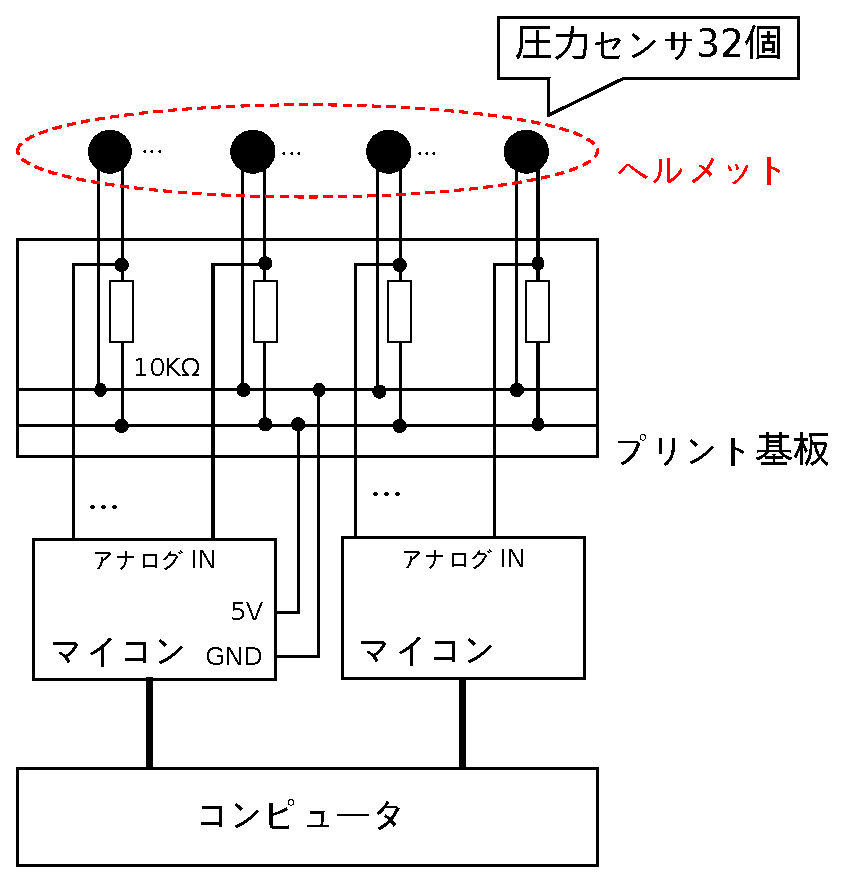
\includegraphics[width=0.65\linewidth]{figure/device.eps}
  \end{center}
  \caption{デバイスの構成}
  \label{device}
\end{figure}

\begin{figure}[!t]
  \begin{center}
    \includegraphics[width=0.6\linewidth]{figure/met_over.eps}
  \end{center}
  \caption{デバイスの外観}
  \label{met_over}
\end{figure}

圧力値を正しく取得するには,センサとヘルメット装着者の頭部が密着している必要があるため,密着度の高いフルフェイス型ヘルメット(B\&B社製BB100)を用いた.圧力センサとしてインターリンクエレクトロニクス社製のFSR402およびFSR402 ShortTailを合計32個使用した.マイコンとしてArduino MEGA2560 R3を使用した.
使用したヘルメットはフリーサイズであり,内装の脱着が困難であったため,\figref{met_in}に示すように頭頂部の内装を取り外して,新たに厚みのあるウレタンスポンジを取り付けた.また,\figref{sensor}に示すようにウレタンスポンジの中央部に切り込みを入れて圧力センサを挿し込んだ.圧力センサは頭頂部に4個,頭頂部周囲に16個,後頭部に6個,左右チークパッド部に6個の合計32個を搭載した.配線はヘルメットの頭頂部にドリルで開けた穴から,ヘルメット外部に取り付けた10K$\Omega$の抵抗を配線してあるプリント基板を経由して,Arduino MEGA2560 R3の5V電源,GND,アナログ入力ポートに接続した.ヘルメット外部に取り付けたプリント基板を\figref{print}に示す.プリント基板はヘルメットのシールド固定用に開けられたネジ穴を用いて左頬部分にボルトで固定しており,取り外しが可能である.

\begin{figure}[!t]
  \begin{center}
    \includegraphics[width=0.6\linewidth]{figure/met_in.eps}
  \end{center}
  \caption{デバイスの内部}
  \label{met_in}
\end{figure}

\begin{figure}[!t]
  \begin{center}
    \includegraphics[width=0.6\linewidth]{figure/sensor.eps}
  \end{center}
  \caption{圧力センサセンサの実装方法}
  \label{sensor}
\end{figure}

\begin{figure}[!t]
  \begin{center}
    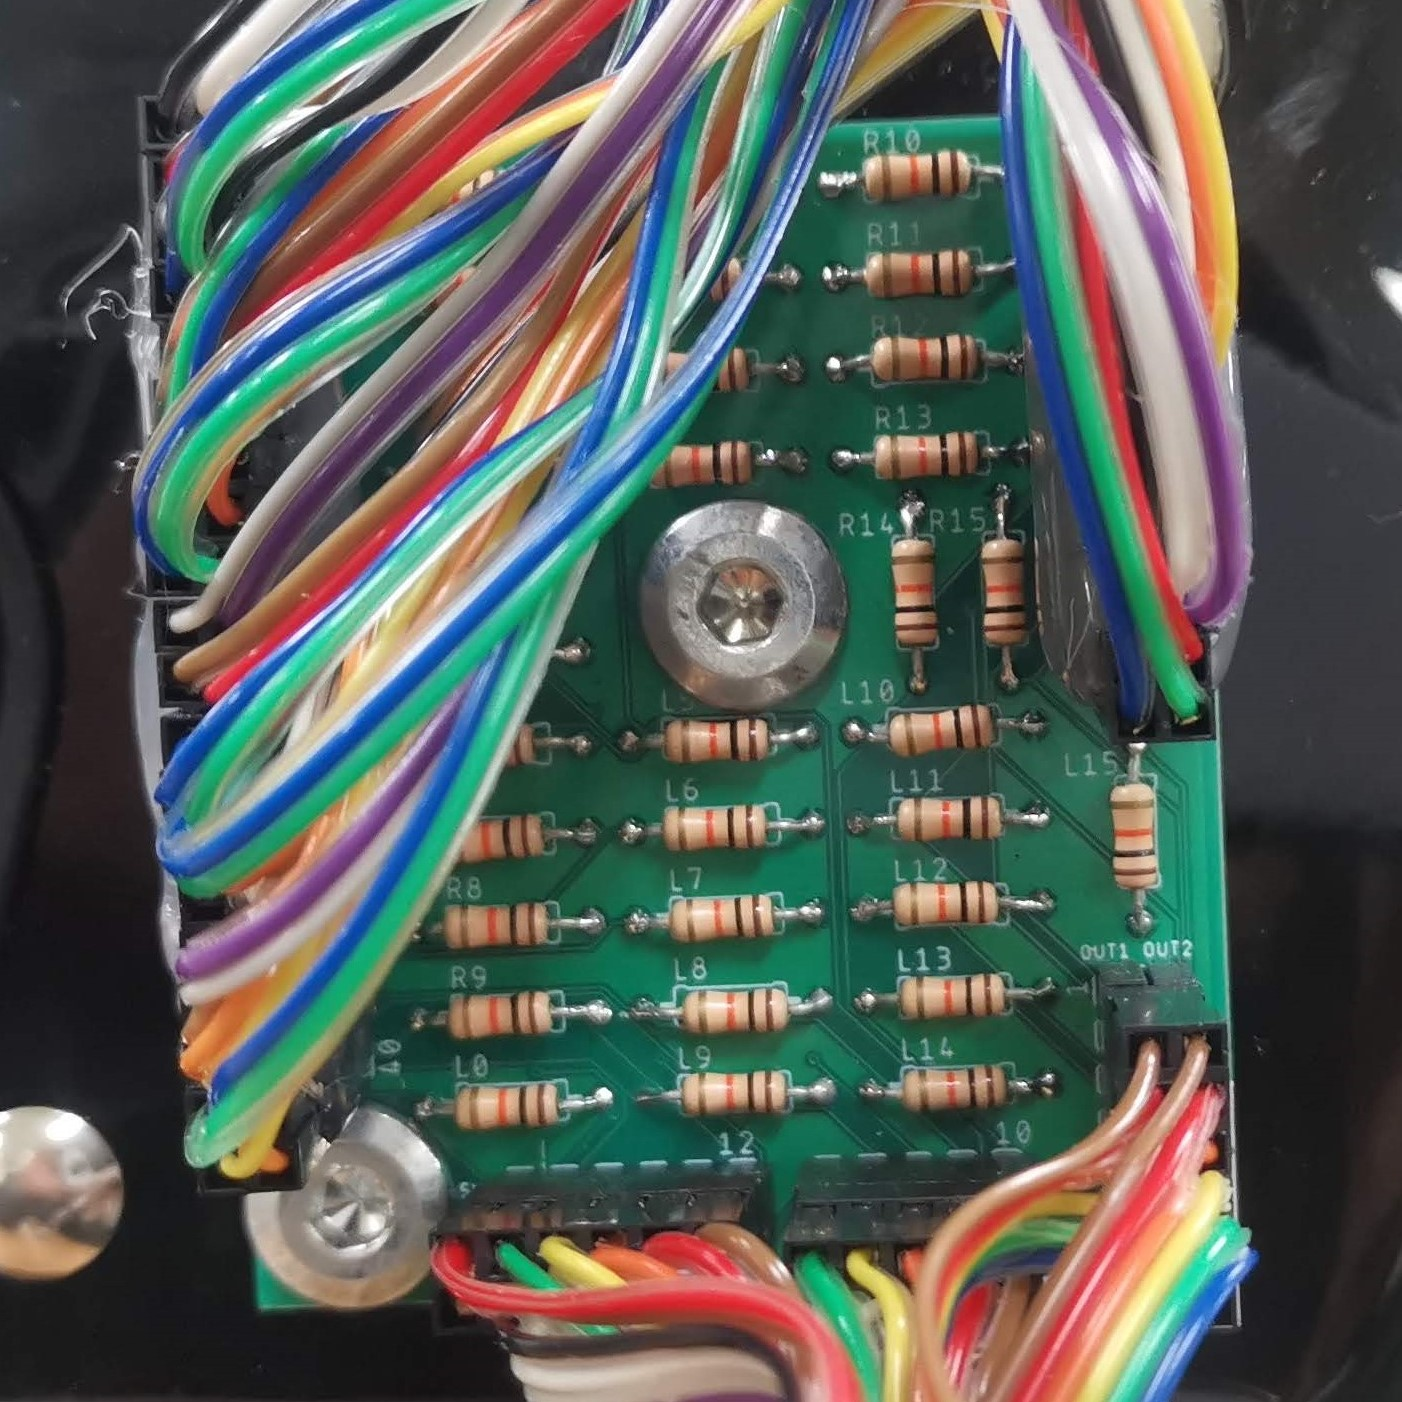
\includegraphics[width=0.6\linewidth]{figure/print.eps}
  \end{center}
  \caption{32個の圧力センサと接続するプリント基板}
  \label{print}
\end{figure}


\subsection{個人識別手法}
%時刻$t$において32次元のデータ$p(t)=[p_0,\dots,p_{31}]$を取得する.
%\textcolor{red}{32次元のデータがとられてからの処理が分からない.ある瞬間の32次元をそのままSVMに入力してその一瞬のデータに対する判定のみで認証をおこなうのか.SVMはどういうカーネルを用いるのか.平均をとるなどの前処理はしているのか,そうならウィンドウサイズは.各種パラメータ類.ソフトウェアのところに書いてる実装についてもここに入れてよい.どういうタイミングで結果を出すのか.複数顔の多数決とか?個人識別,本人認証ともに詳細に書く.データ,処理,特徴量等はすべて変数を用いて厳密かつ正確に書く.}
%ベクトルの特徴の解析と分類には,機械学習の手法であるSupport Vector Machineを用いた.Support Vector Machineは,分類や回帰へ適用できる教師あり学習を用いるパターン認識モデルの一つである.

複数人がシステムに登録されており,その中からヘルメットを装着した人物を識別する手法では,機械学習アルゴリズムの一つであるSupport Vector Machine(SVM)を用いる.SVMは分類や回帰へ適用できる教師あり学習を用いるパターン認識モデルである.提案手法では登録者でラベル付けしたデータを事前に収集してSVMを学習させておき,その後,登録者のうち1名のデータを入力して登録者を識別する.

データの取得はユーザがヘルメットを装着することで開始する.ヘルメットを装着していない状態ではすべての圧力センサの電圧値がほぼ5Vである.ヘルメットの装着時に圧力センサの電圧値が下降し,値が安定した時刻$t=T_s$[s]から2秒間の32個の圧力センサデータ$p(t)=[p_{0,t},\dots,p_{31,t}]$を取得する.この32次元のデータから次元ごとに2秒間に得られたデータの$N$サンプルの平均値$x(t)=\frac{1}{N}\sum_{t=T_S}^{T_S+N-1}p(t)$を計算し,1つの32次元のベクトルを特徴量として得る.
事前に$m$回ヘルメットを被って学習データ$[\bm{x}_i,y_i]$ $(i=1,\dots, m)$を収集し,SVMを学習させる.ただし,$y$は登録者ラベル(登録者名や登録者番号など)である.
そして,識別したいユーザの入力データ$\bm{x}$をSVMに入力し,識別結果$\hat{y}$を得る.
本手法では線形SVMを使用し,パラメータは初期値である$C=1.0$とした.
%\textcolor{red}{本当はパラメータ探さないといけないので,これはまずいけどとりあえずいいかな.}

\subsection{本人認証}
\subsubsection{登録データとの距離計算}
本人認証とは,1人以上の利用者がシステムに登録されており,登録されている人がヘルメットを装着した場合は本人であると認証し,登録されていない人がヘルメットを装着した場合は他人であるとして拒否する手法である.提案手法では,本人認証したい利用者の学習データと未知の装着者の入力データの距離計算方法として,マハラノビス距離を用いる.マハラノビス距離とは多変数間の距離計算手法のひとつであり,データの分布を考慮して正規化した距離を計算できる.

データの取得は個人識別の場合と同様に,ヘルメットの装着時に圧力センサの電圧値が下降し,値が安定した時刻$t=T_s$[s]から2秒間の32個の圧力センサデータ$p(t)=[p_{0,t},\dots,p_{31,t}]$を取得する.この32次元のデータから次元ごとに2秒間に得られたデータの$N$サンプルの平均値$x(t)=\frac{1}{N}\sum_{t=T_S}^{T_S+N-1}p(t)$を計算し,1つの32次元のベクトルを特徴量として得る.

事前に$m$回ヘルメットを被って学習データ$[\bm{x}_i,y_i]$ $(i=1,\dots, m)$を収集する.ただし,$y$は登録者ラベル(登録者名や登録者番号など)である.
学習データの平均値ベクトル$\bm{\mu}$と分散共分散行列$\bm{\Sigma}$を次式で求める.
\begin{eqnarray}
  \bm{\mu} &=& \frac{1}{m}\sum_{i=1}^{m}\bm{x}_i \\
  \bm{\Sigma} &=& \frac{1}{m}\sum_{i=1}^{m}(\bm{x}_i-\bm{\mu})(\bm{x}_i-\bm{\mu})^T
\end{eqnarray}
識別したいユーザの入力データ$\bm{x}$とする.
このとき,入力データが事前に登録された本人のデータであれば,入力データ$\bm{x}$と学習データ$\bm{x}_i$は同じ分散共分散行列$\bm{\Sigma}$の確率分布に従うため,入力データ$\bm{x}$と学習データ$\bm{x}_i$のマハラノビス距離は
\begin{eqnarray}
  d(\bm{x},\bm{x}_i) = \sqrt{(\bm{x}-\bm{x}_i)^{T}\bm{\Sigma}^{-1}(\bm{x}-\bm{x}_i)}
\end{eqnarray}
と定義できる.
%\textcolor{red}{今回登録者は1名?複数人登録されている場合,分散共分散行列は個人ごとに出して,個人ごとに認証判定して,登録者のうち誰かとして認証されればOKってかんじ?}

\subsubsection{認証判定}
閾値を$\theta$とおき,
\begin{equation}
\label{eqn:authentication}
  \theta \geq min_i(d(\bm{x},\bm{x}_i))~(i=1,\dots,m)
\end{equation}
を満たす場合,入力データ$\bm{x}$は登録されているいずれかの所有者から得られたデータであると判定し認証する.
式\ref{eqn:authentication}を満たさない場合,入力データ$\bm{x}$は登録されているいずれの所有者でもない人物のデータであると判定し拒否する.

\subsection{ソフトウェア}
Arduino MEGAのプログラムはArduino IDEで実装した.Arduino MEGAからのデータを受信してcsv形式で保存するコンピュータのプログラムはPythonで実装した.
保存したデータの解析プログラムはPythonで実装した.

個人識別では,事前に収集したセンサデータのcsvファイルを読み出し,sklearn.svm.SVCを用いて学習と識別を行う.sklearn.svm.SVCとは標準的なソフトマージンSVMを実装したscikit-learn\cite{scikit-learn}のライブラリである.また,評価のために交差検証を行うライブラリである,sklearn.model\_selection.cross\_val\_scoreを使用した.

本人認証では,事前に収集したセンサデータのcsvファイルを読み出し,sklearn.covariance.MinCovDetを用いて分散共分散行列を計算する.分散共分散行列の逆行列から,scipy.spatial.distanceを用いてすべての学習データ$\bm{x}_i$に対する入力データ$\bm{x}$のマハラノビス距離を計算する.sklearn.covariance.MinCovDetとは,異常値に対して頑健な分散共分散行列の推定アルゴリズムであるMinimum Covariance Determinant(MCD)を高速化したFast-MCD\cite{fast_mcd}を実装したscikit-learnのライブラリである.また,scipy.spatial.distanceとは,さまざまな距離計算の関数を実装したSciPy\cite{scipy}のライブラリである.

\section{評価}
\label{evaluation}
本節では,提案手法の有効性を評価するために行った実験について説明する.

\subsection{データ収集}
被験者9名(A$\sim$I,全員男性,平均年齢23歳)に\ref{method}節で実装したヘルメットを装着させ,サンプリングレート約30Hzでセンサデータを収集した.
2秒間装着してデータを採取し,取り外して再び2秒間装着してデータを採取する試行を1セット(2サンプル)として,日を変えて10セット,合計で2秒$\times$20サンプル$\times$9人のデータを収集した.
ヘルメットの装着具合の変化にともなうセンサと頭部のさまざまな位置関係のデータを収集するために,セット間に30分以上の休憩時間を設けた.また,データの収集は1人あたり1日最大4セットとした.

\subsection{個人識別}
\subsubsection{評価環境}
収集したデータに対して,各被験者のデータの80\%(16サンプル)を学習させ,20\%(4サンプル)をテストデータとする5分割交差検証によって評価した.使用するセンサの個数による影響も調査するため,1個使用する場合から32個使用する場合までのすべてのセンサの組合せにおいて前述の試行を行った.

また,工事現場などで使用されるハーフ型ヘルメットを想定し,32個のセンサのうち頭頂部の4個と頭頂部周囲の16個の合計20個のセンサに限定して,同様に1個使用する場合から20個使用する場合までの全てのセンサの組合せにおいて評価した.本評価では,32個のセンサを使用する場合をフルフェイス型ヘルメット,20個のセンサを使用する場合をハーフ型ヘルメットと呼ぶ.

\subsubsection{結果と考察}
フルフェイス型ヘルメットでの個人識別の精度を\tabref{full_num}に示す.センサ数が32個の場合は,32個すべてを使用する1通りでの精度であり,センサ数が31個の場合は,32個のうち31個を使用する$_{32}C_{31}=$32通りの中で最も高かった精度である.ここで,センサ数が32個および31個の場合の精度を評価したところ1.00であったため,センサ数を1個から増やしていき,精度が1.00に到達するところまでを評価した.

結果より,センサ数が5個のとき,9人の識別に100\%の精度で成功した.センサ数が4個で99.4\%,3個で97.2\%,2個で92.2\%と高い精度が得られたが,センサ数が1個では60\%と大幅に下がった.

\begin{table}[!t]
  \centering
  \caption{フルフェイス型ヘルメットにおいてセンサ数を1個から32個まで変化させた場合の個人識別精度}
  \begin{tabular}{c|c} \hline\hline
    センサ数 & 精度 \\ \hline
    32 & 1.000 \\
    31 & 1.000 \\
    \vdots & \vdots \\
    5 & 1.000 \\
    4 & 0.994 \\
    3 & 0.972 \\
    2 & 0.922 \\
    1 & 0.600 \\ \hline
  \end{tabular}
  \label{full_num}
\end{table}

% フルフェイス型ヘルメットを想定した場合の結果は,計算量が膨大であったため\textcolor{green}{32$\sim$21個,5$\sim$1個}の場合のみを計算した.\textcolor{green}{5個}の時点でも精度が1.0であったため,\textcolor{green}{20$\sim$6個}の場合の精度も1.0となると仮定した.\par

% フルフェイス型ヘルメットを想定し,全てのセンサから減少させて検証した結果を表\ref{full_num},図\ref{Acc}に示す.また,工事現場などで使用されるハーフ型ヘルメットを想定し,頭頂部の4個と頭頂部周囲の16個のセンサから減少させて検証した場合の結果を表\ref{half_num},図\ref{Acc}に示す.

ハーフ型ヘルメットでの個人識別の精度を\tabref{half_num}に示す.この結果もフルフェイス型ヘルメットと同様にセンサ数が20個および19個の場合の精度を評価したところ1.00であったため,センサ数を1個から増やしていき,精度が1.00に到達するところまで評価した.

結果より,センサ数が5個のとき,9人の識別に100\%の精度で成功した.センサ数が4個,3個,2個の場合では99.4\%,96.7\%,90.0\%と高い精度が得られたが,センサ数が1個では60\%と大幅に下がった.

\begin{table}[!t]
  \centering
  \caption{ハーフ型ヘルメットにおいてセンサ数を1個から20個まで変化させた場合の個人識別精度}
  \begin{tabular}{c|c} \hline\hline
    センサ数 & 精度 \\ \hline
    20 & 1.000 \\
    19 & 1.000 \\
    \vdots & \vdots \\
    5 & 1.000 \\
    4 & 0.994 \\
    3 & 0.967 \\
    2 & 0.900 \\
    1 & 0.600 \\ \hline
  \end{tabular}
  \label{half_num}
\end{table}

これらの結果より,本実験で使用したデータセットに対して,フルフェイス型ヘルメットおよびハーフ型ヘルメットのどちらにおいても,センサ数5個で100\%の精度で識別できることを確認した.しかしながら,登録者数が増加した場合,高い精度を得るためには必要となるセンサ数が増加すると考えられる.
%このように,本実験環境では良い結果が得られた.今後は,より実環境に近い条件で評価していく必要がある.

%\textcolor{red}{表かグラフのどちらか一方でよい.どちらかというと表のほうがよいかな.}
% \begin{figure}[!t]
%   \centering
%     \includegraphics[width=0.70\linewidth]{figure/Acc.eps}
%   \caption{精度の変化}
%   \label{Acc}
% \end{figure}

\subsection{本人認証}
\subsubsection{評価環境}
収集したデータのうち,1名の被験者を本人,残り8名の被験者を他人として,本人としたデータの80\%(16サンプル)を学習データとして登録し,残り20\%(4サンプル)をテストデータとして5分割交差検証を行い本人の認証精度を計測した.さらに,交差検証で使用した5パターンの学習データに対して,他人とした8名すべてのデータ(160サンプル)を用いて他人の認証精度を計測した.また,本人を9名全員ローテーションして評価した.\par

認証精度の評価指標として,FRR,FAR,EERを用いる.FRR(False Reject Rate:本人拒否率)は本人を他人であると誤って判断し拒否する割合である.
FAR(False Accept Rate:他人受入率)は他人を本人であると誤って判断し認証する割合である.
認証するか否かを決定する閾値を小さく設定するほど認証判定が厳密になるためFRRが増加し,対して閾値を大きく設定するほど認証判定が緩くなるためFARが増加する.
FRRとFARはトレードオフの関係にあり,FRRとFARが同値になるときの値をEER(Equal Error Rate:等誤り率)と呼ぶ.通常,本人認証手法の性能評価においてはEERの値が指標として用いられ,EERが小さいほど性能が良いとされる.

\subsubsection{結果と考察}
各被験者のEERを\tabref{EER_num}に示す.
また,閾値を変化させたときの各被験者のFRRとFARを\figref{EER}に示す.
Totalは被験者全員の平均を示している.
\tabref{EER_num}より被験者A,E,G,IのEERはおおよそ0.01以下と良い結果が得られた.これは,検証に用いたデータセットにおいて,本人は100回に1回以下の割合で認証に失敗し,他人は100回に1回以下の割合で認証を突破することを意味している.文献\cite{face_auth}において,顔認証のEERが0.012であると報告されていることを考慮すると,これらの被験者については同等の性能が得られたといえる.\figref{EER}より,被験者Eについては,閾値が他の被験者よりも大きい60程度でFRRとFARが交差している.これは収集した圧力データのサンプルに外れ値が存在したため,外れ値を正しく認証するために閾値を大きくする必要があったためである.\par

\begin{table}[!t]
  \centering
  \caption{本人認証における各被験者および全被験者平均のEER}
  \begin{tabular}{c|c} \hline\hline
    被験者 & EER \\ \hline
    A & 0.002 \\
    B & 0.095 \\
    C & 0.050 \\
    D & 0.055 \\
    E & 0.006 \\
    F & 0.094 \\
    G & 0.012 \\
    H & 0.050 \\
    I & 0.000 \\ \hline
    Total & 0.076 \\ \hline
  \end{tabular}
  \label{EER_num}
\end{table}

\begin{figure}[!t]
  \centering
    \includegraphics[width=1\linewidth]{figure/EER.eps}
  \caption{本人認証における各被験者および全被験者平均のFRRとFAR}
  \label{EER}
\end{figure}

次に精度が良い被験者はC,D,Hであり,EERはおおよそ0.05である.ここで精度の低下の要因を究明するために,収集したすべてのデータに対して主成分分析を行い,第一主成分および第二主成分の2次元に圧縮したデータを2次元平面上にプロットし,目視で確認した.結果を\figref{PCA}に示す.\figref{PCA}より,被験者Cについて見ると,被験者Cのデータ群のうち1サンプルが被験者Iのデータ群と近い位置にあるが,他の被験者のデータ群との重なりは見られない.しかしながら,第一主成分方向の分散が大きい.一方,被験者D,Hのデータ群は互いに大きく重なっており,両者が影響し合って精度が低下したと考えられる.\par

\begin{figure}[!t]
  \centering
    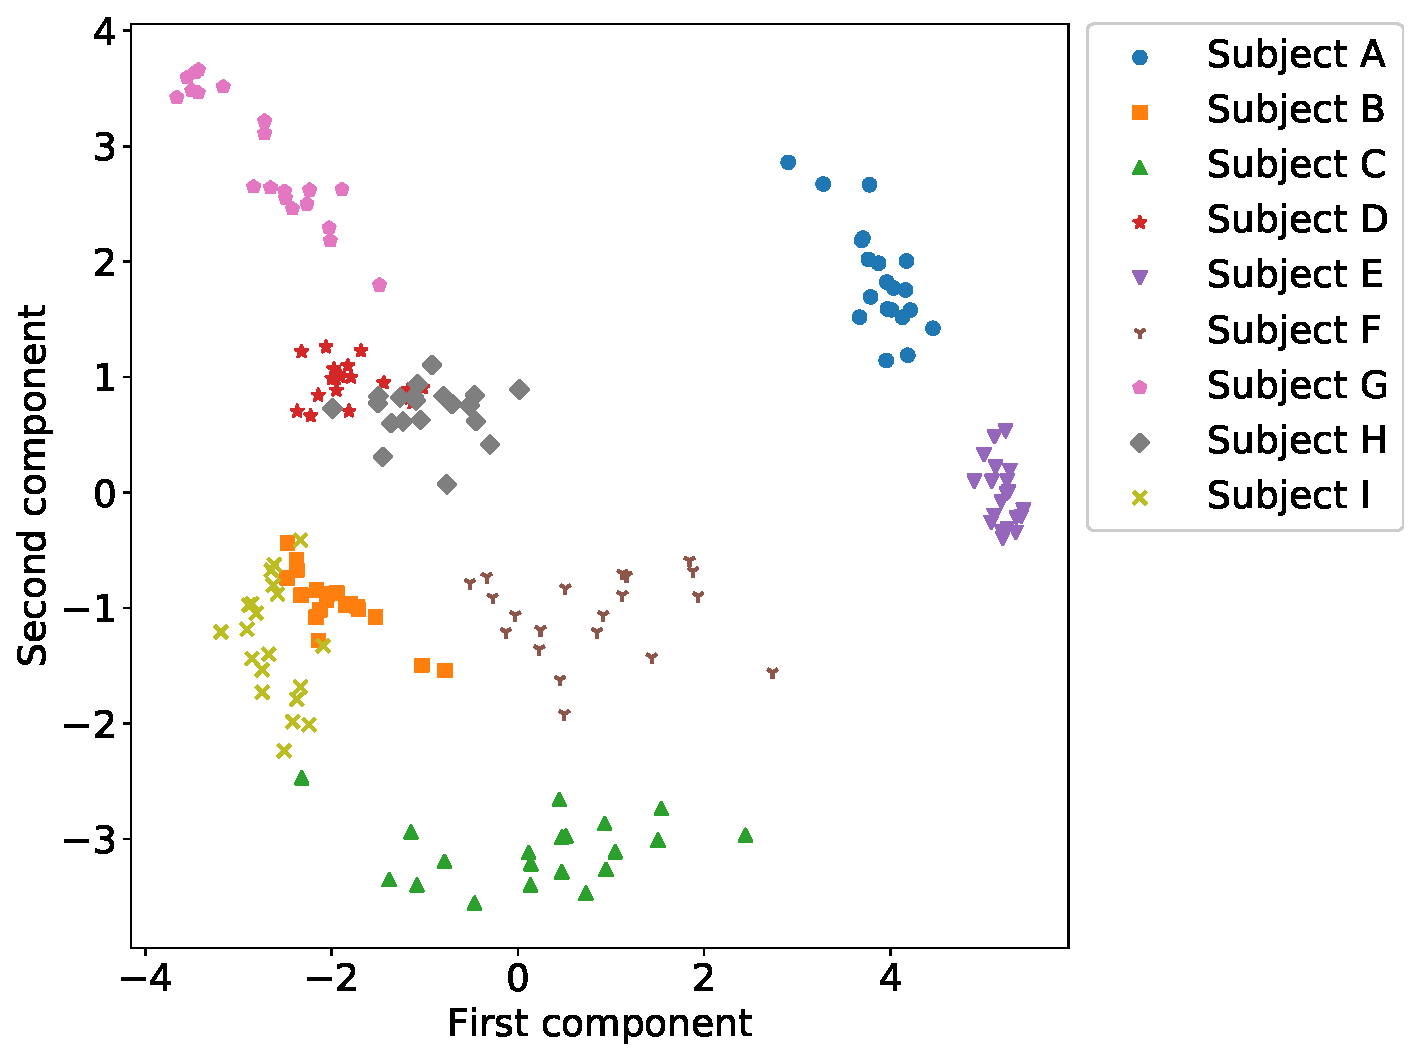
\includegraphics[width=1\linewidth]{figure/PCA.eps}
  \caption{32次元の特徴量をPCAによって2次元に圧縮した主成分の分布}
  \label{PCA}
\end{figure}

最も精度が悪かった被験者はB,Fであり,これらの被験者のEERはおおよそ0.095であった.被験者Bのデータ群は分散が小さいが,被験者Iのデータ群との重なりが見られる.しかしながら,検証に用いたデータセットにおける被験者IのEERは0であり,誤りなく判別ができていた.したがって,これらのデータ群の重なりは主成分分析で2次元に圧縮した際のデータの損失による影響だと考えられる.一方,被験者Fのデータ群は他の被験者のデータ群との重なりが見られないが,第一主成分と第二主成分の両方向の分散が大きい.主成分分析によるデータ圧縮の影響を考慮すると,32次元のデータでは他の被験者のデータ群との重複が推察される.被験者Fのデータの散らばりに影響されて,被験者Fのデータ群の近くに位置する被験者B,Cの精度も低下したと考えられる.特に,被験者Bは2サンプルが被験者Fのデータ群と近い位置に存在するため,被験者Cに比べて精度が低下したと考えられる.\par

被験者全員の平均EERは約0.076であった.被験者ごとのEERに差が見られたことから,より多くの被験者のデータを用いて検証する必要がある.また,提案手法は学習データと入力データの距離を用いて認証を行うため,学習データ数をさらに増やすことで精度の改善が見込まれる.
このほか,ヘルメットを装着する一連の流れにおける時系列圧力データを用いて認証する手法についても今後検証する.

\section{おわりに}
\label{conclude}
本研究では,圧力センサを内部に取り付けたヘルメットを装着することで頭部の形状を計測して,頭部形状の個人差から個人を識別する手法を提案し,プロトタイプデバイスの実装と評価を行った.プロトタイプデバイスは市販のフルフェイス型ヘルメットを加工し,圧力センサを取り付けた.評価では,プロトタイプデバイスからデータを取得するためにデータ収集プログラムを作成し,頭部形状データとして被験者9人からそれぞれ2秒間のセンサ値を20回分取得した.複数の登録者のうち誰が装着したのかを判別することを目的とした個人識別と,二輪車の鍵のように用いることを想定して1名の登録者であるか他人であるかを判別することを目的とする本人認証を行った.

%個人識別ではSupport Vector Machineを用いて学習,識別し,交差検証を行い精度を評価した.本人認証では,登録データと入力データのマハラノビス距離を計算し,本人認証するか拒否するかの閾値を移動させて認証性能を評価した.
評価実験では,個人識別では非常に精度が高かったため,識別に使用するセンサ数を減少させて識別精度がどのように変化するかを検証した.その結果,本実験で使用したデータセットに対して一番効率の良いセンサ数は,フルフェイス型ヘルメットおよび,ハーフ型ヘルメットのどちらの場合も5個であった.本人認証では認証の精度の評価指標であるEERが9名中4名が0.012以下,平均0.076という結果が得られた.これらの結果より,本手法は個人識別手法として有効であると考えられる.今後はさらなるデータの収集を行い,実環境での提案手法の評価を行う.

\bibliography{references}
\bibliographystyle{junsrt}

\end{document}
